\subsection{観測カテゴリモデルによる同時推定}
\label{sec:observed-category-simulation}
本小節では，$W,Z\to F\to Y_j$の測定構造を維持し，欠測を含む観測カテゴリを
利用する別の識別経路を検討する。各block lawを先に回復するのではなく，
複数の応答patternに共通する測定核と混合比率を用い，欠測機構と潜在構造を
同時に推定する。したがって，以下の数値は第4節のbridge-weighted estimatorの
性能評価ではない。

\noindent\textbf{生成モデル.}
$X=x$を固定し，常時観測される$V=(W,Z)$は二値の$W,Z$からなる4カテゴリとする。
$F\in\{1,2\}$は単一の有限カテゴリ因子，$Y_1,Y_2,Y_3$は二値itemとし，$Y_1$は常時観測する。
$V$の4セルを$(0,0),(0,1),(1,0),(1,1)$の順に並べ，
\begin{equation}
\begin{aligned}
P(V=v)&=1/4,\\
\{P(F=2\mid V=v)\}_v&=(0.10,0.30,0.60,0.80)
\end{aligned}
\label{eq:oc-v-lambda}
\end{equation}
と置く。従って$(p_1,p_2)=(0.55,0.45)$である。
$M_j(y,f)=P(Y_j=y\mid F=f)$とし，$M_j(1,f)$は式
\eqref{eq:simulation-measurement-kernel}と同じ6成分を用いる。
有限クラスのproduct measurement modelはAllman et al. (2009, Sections 3--4)の
モデル族に対応するが，数値設定は本研究で定めたものである。

応答確率を$\pi_j(a,y)=P(D_j=1\mid Y_1=a,Y_j=y)$とし，
同時分布を
\begin{equation}
\begin{aligned}
p(v,f,y,d)
&=p(v)\lambda_f(v)\prod_{j=1}^{3}M_j(y_j,f)\,
\mathbf1\{d_1=1\}\\
&\quad\times\prod_{j=2}^{3}\pi_j(y_1,y_j)^{d_j}
\{1-\pi_j(y_1,y_j)\}^{1-d_j}
\end{aligned}
\label{eq:oc-dgp}
\end{equation}
とする。式\eqref{eq:oc-dgp}は$V$から$F$，$F$から各$Y_j$を生成する。
測定核には$W,Z$の直接効果を入れず，$D_2,D_3$は$Y$の下で条件付き独立とする。
各$D_j$には$Y_1,Y_j$以外の$F,V$や他の欠測itemの直接効果を入れない。
これは一般のMissing-IV exclusionより強い制約である。

MCARでは$\pi_j=0.70$，MARでは
$\operatorname{logit}\pi_j=\alpha_j-0.50Y_1$，MNARでは式
\eqref{eq:simulation-missingness}を用いる。切片は母集団上で較正し，
$Y_2,Y_3$の平均観測率を各0.70，3項目平均を0.80とする。
標本サイズは$n=1{,}000$，各機構で100 Monte Carlo replicationsとし，
機構間では完全データと応答乱数を共有する。
実現した平均item観測率はMCAR，MAR，MNARの順に0.8003，0.7998，0.7994，
complete-case率は0.4907，0.4926，0.5202であった。
条件付き独立な応答とpositivityの下ではcomplete-case確率は正であり，
global complete caseが存在しない設計への適用は本実験では検証しない。

\noindent\textbf{識別条件の確認.}
$T_j$を，$D_j=1$なら観測値0または1，$D_j=0$なら欠測カテゴリ$\mathrm{mis}$を取る
常時観測の3カテゴリ変数とする。$Y_1=a$で層別すると，
$T_2,T_3,V$は$F$の下で条件付き独立であり，
\begin{equation}
\begin{aligned}
&P(T_2=t_2,T_3=t_3,V=v\mid Y_1=a)\\
&\quad=\sum_{f=1}^2\omega_f(a)
K_{2f}^{(a)}(t_2)K_{3f}^{(a)}(t_3)G_f(v)
\end{aligned}
\label{eq:oc-tensor}
\end{equation}
と書ける。ここで$\omega_f(a)=P(F=f\mid Y_1=a)$，
$G_f(v)=P(V=v\mid F=f)$，$K_{jf}^{(a)}$は$T_j\mid(F=f,Y_1=a)$の確率列である。
$G_f$の使用はBayes分解であり，生成DAGの辺を逆転させるものではない。

応答確率のpositivity，$M_2,M_3$のclass間差，および$\lambda_f(v)$の変動により，
$K_2^{(a)},K_3^{(a)},G$のcolumn Kruskal rankは全て2となる。
Allman et al. (2009, Section 4, Theorem 1 and Corollary 2)の条件
$2+2+2=2r+2=6$を満たす。
観測値のカテゴリでは$K_{jf}^{(a)}(y)=\pi_j(a,y)M_j(y,f)$なので，
\begin{equation}
\begin{pmatrix}
K_{j1}^{(a)}(0)&K_{j1}^{(a)}(1)\\
K_{j2}^{(a)}(0)&K_{j2}^{(a)}(1)
\end{pmatrix}
\begin{pmatrix}\pi_j(a,0)^{-1}\\\pi_j(a,1)^{-1}\end{pmatrix}
=\begin{pmatrix}1\\1\end{pmatrix}
\label{eq:oc-normalization}
\end{equation}
から応答確率と測定核を分離できる。係数行列の行列式は
$\pi_j(a,0)\pi_j(a,1)\{M_j(1,2)-M_j(1,1)\}\ne0$である。
$M_2(1,1)<M_2(1,2)$で各層のlabelをそろえれば，
$p_f=\sum_aP(Y_1=a)\omega_f(a)$と
$M_1(a,f)=P(Y_1=a)\omega_f(a)/p_f$も得られる。

母集団テンソルだけを入力したmatrix-pencil分解と式
\eqref{eq:oc-normalization}の逆算により，$M_j,\pi_j,G,p_f$を絶対誤差
$10^{-9}$未満で回復した。MNARの$K_2$の最小特異値は層ごとに0.4106，0.3489，
$K_3$は0.5428，0.4604，$G$は0.3838であった。
一方，4セルの任意のblock lawに対する条件付き行列のrankは2であり，
必要なrank 4を満たさない。本実験の識別経路を命題2.1のblockwise
complete-case completenessと同一視することはできない。

\noindent\textbf{推定と比較手法.}
候補推定量は，$O_i=(Y_{1i},V_i,T_{2i},T_{3i})$について，$V_i$を条件とした観測尤度
\begin{equation}
L_{\rm OC}(\theta)=\prod_{i=1}^n
\left\{\sum_{f=1}^2\lambda_f(V_i)M_1(Y_{1i},f)
\prod_{j=2}^3K_{jf}^{(Y_{1i})}(T_{ji})\right\}
\label{eq:oc-likelihood}
\end{equation}
を最大化する。$M_j$，$\lambda_f(v)$，$\pi_j(a,y)$は各有限セル上で推定し，
$K_{jf}^{(a)}(\mathrm{mis})=1-\sum_{y=0}^1\pi_j(a,y)M_j(y,f)$とする。
欠測値と$F$を和で消去し，全応答patternを同時に用いる。測定核の共通性を課す点が，
blockごとの任意の分布を別々に推定する方法と異なる。

比較は四手法とする。complete-data oracle (O)は欠測前の全$Y$から$F$を推定する。
Ignorable FIML (I)はselectionを無視し，MCAR・MARでは正指定，MNARでは誤指定となる。
Restricted selection (R)は$\pi_j$を$Y_j$だけの関数とし，MCARでは正指定だが，
MAR・MNARでは$Y_1$効果を落とした誤指定である。
Candidate saturated (C)は各$\pi_j(a,y)$を4セル自由に推定する。
全手法で同じ$V$情報を使用する。なお，二値の$Y_1,Y_j$では，切片・両主効果・
交互作用を含むlogisticは飽和4セルと一対一対応するため，正指定selection likelihoodと
候補法を別々の手法として比較しない。

6個の乱数初期値から最も大きい尤度の解を選び，真値は初期値に用いない。
logit parameterを$[-10,10]$に制限し，絶対値9.9以上を境界付近と記録する。
反復上限は1,500である。推定SEには，$V$の経験分布の推定誤差も含めたsandwichと
delta法を用いる。第5節のbridge推定量の漸近理論をこの尤度へそのまま適用するものではない。

\noindent\textbf{結果.}
図\ref{fig:oc-outcome}にMNAR下のoutcome平均$\mu_j=P(Y_j=1)$のbiasとSDを示す。
候補法の$\mu_2,\mu_3$のbiasは$-0.0009,0.0029$であり，Iの$-0.0914,-0.0801$，
Rの0.0745，0.0669より絶対値が小さかった。selectionを無視した場合の過小評価と，
$Y_1$効果を除いた場合の過大評価の双方が，候補法では小さくなっている。
一方，SDは候補法で0.0352，0.0288，oracleで0.0146，0.0160であり，
未知のselection確率を同時に推定する変動が残る。

\begin{center}
\begin{minipage}{\linewidth}
\centering
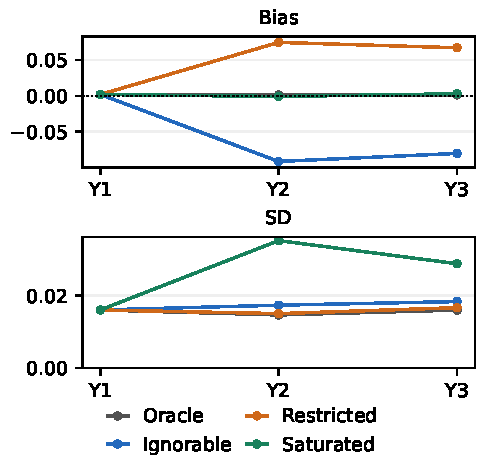
\includegraphics[width=\linewidth]{simulation/observed_category/report_n1000/paper_outcome_point.pdf}
\captionof{figure}{観測カテゴリモデルのMNAR実験，$n=1{,}000$，100反復。
各outcome平均のbiasとSDは全反復から計算する。}
\label{fig:oc-outcome}
\end{minipage}
\end{center}

表\ref{tab:oc-summary}の通り，MNARにおける候補法の測定核6成分の平均絶対biasは
0.0042，成分別RMSEの平均は0.0387であり，Iの0.0718，0.0816およびRの
0.0436，0.0542より小さかった。class 2の$M_2,M_3$のbiasは候補法で
$-0.0117,-0.0052$，Iで$-0.1635,-0.1373$であった。共通測定核と観測カテゴリの
情報を用いることで，欠測によるclass-specificな測定確率の偏りが補正されたと考えられる。
ただし，これは正指定の飽和logistic selectionに対する優位性を意味しない。

\begin{center}
\begin{minipage}{\linewidth}
\centering
\setlength{\tabcolsep}{5pt}
\begin{tabular}{@{}llrrrr@{}}
\hline
機構 & 方法 & $|\mathrm{Bias}|_M$ & RMSE$_M$ & Bias$_p$ & RMSE$_p$\\
\hline
MCAR & O & 0.0023 & 0.0247 & 0.0052 & 0.0256\\
MCAR & I & 0.0030 & 0.0303 & 0.0078 & 0.0328\\
MCAR & R & 0.0026 & 0.0328 & 0.0085 & 0.0332\\
MCAR & C & 0.0035 & 0.0429 & 0.0090 & 0.0345\\
MAR & O & 0.0023 & 0.0247 & 0.0052 & 0.0256\\
MAR & I & 0.0028 & 0.0302 & 0.0092 & 0.0331\\
MAR & R & 0.0364 & 0.0511 & 0.0253 & 0.0410\\
MAR & C & 0.0040 & 0.0444 & 0.0103 & 0.0346\\
MNAR & O & 0.0023 & 0.0247 & 0.0052 & 0.0256\\
MNAR & I & 0.0718 & 0.0816 & -0.0097 & 0.0397\\
MNAR & R & 0.0436 & 0.0542 & 0.0153 & 0.0326\\
MNAR & C & 0.0042 & 0.0387 & 0.0072 & 0.0295\\
\hline
\end{tabular}

\captionof{table}{全100反復の潜在母数の比較。O: oracle，I: ignorable，R: restricted，C: candidate。
$|\mathrm{Bias}|_M$は6成分のbiasの絶対値の平均，RMSE$_M$は成分別RMSEの平均。
$p$の指標はclass 2比率に対する値である。}
\label{tab:oc-summary}
\end{minipage}
\end{center}

MCAR・MARでは，候補法の測定核RMSEは0.0429，0.0444であり，
Iの0.0303，0.0302より大きかった。欠測を無視できる場合には，selectionの追加推定は
効率性の改善を保証しない。MNARの$p_2$のbiasとRMSEは候補法で0.0072，0.0295，
Iで$-0.0097$，0.0397，Rで0.0153，0.0326であり，候補法には有限標本biasが残るものの，
RMSEは両比較法より小さかった。

図\ref{fig:oc-joint}は，推定された測定核とclass比率から構成した$Y$全体の8セル分布を示す。
IとRには$n=1{,}000$でも分布の偏りが見られる一方，候補法の平均推定分布はtruthと
oracleに近かった。このfull joint lawは同時に推定した潜在モデルから得られるものであり，
独立したStage-1 bridgeの回復結果ではない。

\begin{center}
\begin{minipage}{\linewidth}
\centering
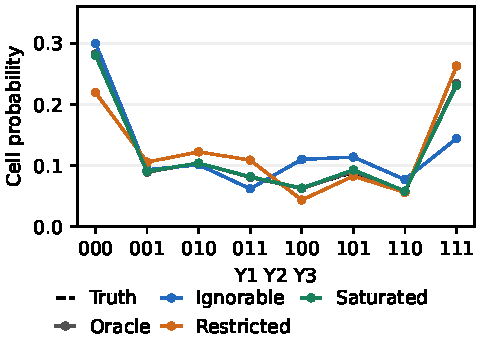
\includegraphics[width=\linewidth]{simulation/observed_category/report_n1000/paper_joint.pdf}
\captionof{figure}{MNARのfull outcome law。横軸は$(Y_1,Y_2,Y_3)$の8セル，
各曲線は100反復の推定確率の平均，破線は母集団の真の確率である。}
\label{fig:oc-joint}
\end{minipage}
\end{center}

\noindent\textbf{区間推定の限界.}
全解が設定した収束判定を満たしたが，候補法の境界付近の解はMCAR，MAR，MNARで
6，6，19反復であった。MNARのIは9反復，Rは100反復が境界付近であった。
境界付近，非収束，またはHessian非正定値の反復には通常のWald区間を付与しない。
従ってMNARで候補法のCIが得られたのは81/100反復であり，
その部分標本における$\mu_2,\mu_3,p_2$のcoverageは0.975，0.963，0.951であった。
この値を全100反復での名目95\%達成と解釈してはならない。

\begin{center}
\begin{minipage}{\linewidth}
\centering
\begin{tabular}{@{}lrrrrr@{}}
\hline
対象 & Bias & SD & SE & Cov. & $B_{\rm CI}$\\
\hline
$M_2(1,2)$ & -0.0117 & 0.0478 & 0.0525 & 1.000 & 81\\
$M_3(1,2)$ & -0.0052 & 0.0411 & 0.0428 & 0.975 & 81\\
$p_2$ & 0.0072 & 0.0288 & 0.0331 & 0.951 & 81\\
$\mu_2$ & -0.0009 & 0.0352 & 0.0400 & 0.975 & 81\\
$\mu_3$ & 0.0029 & 0.0288 & 0.0329 & 0.963 & 81\\
\hline
\end{tabular}

\captionof{table}{MNARでの候補法の推論。BiasとSDは全100反復，SEとCov.は
有効な$B_{\rm CI}$反復のみ。境界付近の19反復を除外して点推定のbiasを計算したものではない。}
\label{tab:oc-inference}
\end{minipage}
\end{center}

有効な81反復だけにそろえた$\mu_2,\mu_3$のSDは0.0347，0.0272であり，
平均推定SEの0.0400，0.0329はこれらより大きかった。境界解の減少と，内点でのSEの較正は
別々に検討する必要がある。候補法はMNARの点推定を改善したが，
安定した区間推定には境界を扱う手法の検討が残る。新規性，漸近理論，および測定族・
応答の条件付き独立性を誤指定した場合の頑健性は，本実験だけからは主張しない。
